\documentclass[a4paper]{article}

\usepackage{hyperref}
\hypersetup{
colorlinks=false, % bool: Liens colorés
pdfborder={0 0 0} % Ne pas encadrer les liens
}
\usepackage[utf8]{inputenc}
\usepackage[francais]{babel}
\usepackage[top=2cm, bottom=2cm, left=2cm, right=2cm]{geometry}
\usepackage{graphicx}
\usepackage[final]{pdfpages}
\usepackage{rotating}
\usepackage{eurosym}
\usepackage{lscape}
\usepackage{float}
\usepackage{color}
\usepackage{colortbl}
% définir les commandes ici

% s'il y a beaucoup de commandes et de packages à inclure n'h&ésitez pas
% à mettre tout ça dans un fichier include.tex et l'inclure
% \input{include.tex}




\begin{document}
\title{PdC 2 : Dossier d'Initialisation}
\author{Elisa ABIDH, Adrien BROCHOT, Martin RICHARD, Jetmir XHEMBULLA}

%------------------------------------- Page de titre
\maketitle
%\begin{titlepage}
%~

%\vfill
%\begin{Large}
%Septembre 2011
%\end{Large}
%\vfill
%\end{titlepage}
%----------------------------------------------------

%--------------------------------- Table des matières
\newpage
\tableofcontents
\newpage
%----------------------------------------------- Plan

\section{Objet du projet - Contexte}

\subsection{Contexte général du projet}

\paragraph{} Le réseau actuel du campus de l'INSA est actuellement limité et en partie vétuste. Notre client, la direction de l'INSA, a donc mis en place un plan de rénovation de ce dernier. Ce projet se place dans ce contexte mais vise avant tout à modifier l'architecture actuelle du réseau afin d'y intégrer la ToIP.
\paragraph{} L'étude portera sur l'intégralité du site principal sur lequel sont déployés les équipements réseaux. L'un des points particuliers de l'infrastructure à définir est la diversité des utilisateurs présents sur le campus. Ce dernier est en effet composé aussi bien de laboratoires de recherches que de résidences, de bibliothèque ou encore de bureaux pour services administratifs de l'INSA. Cette diversité rend l'infrastructure plus compliqués du fait de la multiplicité des usages qui lui sont demandés.
\paragraph{} Sur le campus de l'INSA, les réseaux données et voix sont, à l'heure actuelle, séparés. Cette séparation entraine un problème de gestion évident des deux systèmes de communication entrainant un manque de sécurité et d'efficacité global de l'infrastructure. Leur gestion est actuellement assurée par la direction informatique mais pour le cas du réseau téléphonique, les abonés disposent d'une ligne téléphonique classique et leurs appels sont rétro-facturés.
\paragraph{} L'ajout de fonctions ToIP dans le réseau du campus a pour but une homogénisation des ressources. La gestion des différents réseaux sera alors facilitée et une meilleur maîtrise des coûts de téléphonie. Cela permettra également, lors du rennouvellement des PABX de les passer également en ToIP.

\subsection{Objectifs du projet}
\paragraph{} La mise en place de la téléphonie par IP sur le campus de l'INSA demande une modification globale de l'architecture réseau des équipements du campus. Ce projet a pour but de dégager une solution pour cette migration. L'objectif étant ici d'effectuer un travail de consultant aboutissant à un appel d'offre précisant l'organisation et le déploiement des nouveaux équipement nécessaires.

\paragraph{} Ce projet comporte de multiples objectifs visibles au travers des différents documents et rapports de retour. Il devra permettre à la direction de l'INSA d'appréhender les modifications et les travaux à effectuer sur l'infrastructure réseau du campus. Il doit leur permettre de prendre une décision finale quand au lancement éventuel de l'appel d'offre sur le déploiement qui aura été décrit dans l'étude fournie.

\paragraph{} Ce projet a finalement pour objectif la définition d'une solution complète de réorganisation du réseau du campus de l'INSA permettant d'ajouter des possibilités de ToIP sur le campus. Il devra montrer des solutions techniques et définir une architecture plus fiable, plus sécurisée et plus robuste que celle actuellement utilisée. Il présentera également les budgets nécessaires au déploiement de cette nouvelle architecture ainsi que l'odonnancement des tâches de déploiement à effectuer sur les différentes installations du campus. Il est en effet impossible de négliger le temps de déploiement d'une telle migration lors de l'étude d'une solution.


\newpage
\section{Résultats Attendus}
\paragraph{} Ce projet doit aborder de nombreux aspects lors de l'étude des solutions disponibles. Il doit s'adapter aux différents publics à qui le retour de l'étude sera fait et qui devront décider du déploiement futur de la nouvelle architecture du réseau du campus. Afin d'aborder tous les aspects de manière complète sans pour autant contraindre certains acteurs du futur projet à parcourir des documents très techniques et ne les concernant pas, plusieurs dossiers différents seront rendus, chacun ayant un objectif et un destinataire précis. \\


\subsection{Rapport d'aide décisionelle:} Rapport destiné à un public non technique, il présente la solution retenue lors  des études préliminaires. Il est destiné au client : la direction de l'INSA. Il offre une présentation complète du projet d'amménagement ainsi que la nouvelle architecture (technique, administrative). Une présentation de l'aspect économique et financier de la solution sera également présente dans ce rapport. Il permettra de définir les hypothèses effectuées lors de l'étude sur les moyens à disposition, les caractéristiques de la solution proposée ainsi que les conclusions du groupe d'étude.

\subsection{Dossier d'étude architecturale:} Dossier technique, il définit les technologies retenues lors de l'étude des solutions possibles. Il décrit précisément l'architecture technique du nouveau réseau mis en place sur le campus. Il permet de visualiser le réseau tel qu'il sera au terme du déploiement suivant la solution retenue. Il contiendra de nombreux schémas présentant la nouvelle architecture, la nouvelle organisation générale du campus suite au changement d'infrastructure réseau, les plans de migration de certaines technologies désormais obsolètes et la présentation des éléments les remplaçant. Il ne se limitera pas à l'aspect physique, il présentera également les différents protocoles, et standards utilisés pour l'exploitation de la nouvelle architecture.

\subsection{Rapport d'organisation du déploiement:} Ce rapport décrit l'ensemble du cycle de vie du projet de déploiement depuis son lancement jusqu'à la fin des travaux. Il permet de donner au client  une idée du déroulement des diverses opérations effectuées sur le campus. Ce document est essentiel car il permet de justifier les choix effectués dans la solution de réorganisation du réseau choisie. Il constitue également une étude du mode de déploiement optimal trouvé par notre groupe d'étude pour mettre en place la nouvelle infrastructure réseau du campus en génant un minimum les utilisateurs. Il permet de définir les rôles de chaque structure organisationnelle dans le projet de déploiement (Direction informatique, Direction Générale...).

\subsection{Document de cadrage budgetaire:} Lors de ce projet, de nombreux éléments matériels devront être achetés et installés à divers emplacements du campus. En fonction de l'ordonnancement définit par le rapport d'organisation du déploiement, il convient d'optimiser l'achat de ces équipements afin d'éviter d'avoir à gérer un stock important. Le but étant ici d'éviter l'achat d'équipements trop longtemps avant leur utilisation dans le déploiement du système mais également d'éviter de bloquer le déploiement à cause d'un manque d'équipement. Ce document décrit exhaustivement les tarifs des différents éléments nécessaires à la mise en place de la nouvelle architecture retenue lors de l'étude précédente. Il permet au client de planifier les différentes commandes partielles qu'il aura à effectuer lors du déploiement et de connaître le budget global de la solution proposée

\newpage
\section{Méthodes utilisées et phasage du projet}

\subsection{Méthodes adoptées}
\subsubsection{Ressources}
Pour ce projet, notre groupe d'étude comporte quatre personnes : Adrien BROCHOT, chef de projet, et Elisa ABIDH, Martin RICHARD, Jetmir XHEMBULLA qui constitueront l'équipe technique. A cause du faible effectif de l'équipe, aucun rôle de chef de projet n'est officielement attribué. Le chef de projet contrôlera cependant le respect des démarches qualités lors du rendu de documents.

\subsubsection{Outils utilisés}
\paragraph*{• Le mail:}Outil de communication essentiel dans le travil en équipe à distance, le mail sera principalement utilisé à des fins de plannification de réunions lorsque celles ci n'auront pas été définies lors des périodes de travail au département.

\paragraph*{• Le dépot git:}Afin de mettre en commun les parties/documents rédigés, un dépot git a été créé et servira de centre de données. Tous les membres de l'équipe y auront accès et devront à chaque modification d'un document le mettre à jour sur le dépot.

\paragraph*{• LaTeX:}Lors de ce projet, tous les documents seront écrits en LaTeX

\subsection{Description des phases}

\subsubsection{1: Etude préparatoire} Cette phase a pour objectif de donner à notre groupe d'étude une visibilité approfondie de l'infrastructure du réseau du campus, ainsi que de la solution déployée sur le campus de l'université Lyon 1 qui a subi une migration similaire à celle que nous nous apprettons à plannifier. 

\subsubsection{Phase 2: Analyse décisionnelle} Suite à l'étude préparatoire, nous pouvons commencer à étudier un maximum de solution possibles lors de cette phase. Le but est ici d'envisager et de comparer plusieurs infrastructures. Leur comparaison n'étant pas encore effectuée, il convient de n'oublier aucune technologie possible et de lister un maximum d'équipements adaptés pour avoir un plus large choix lors de la sélection de la solution qui sera par la suite proposée au client. Lors de cette phase, il faut ensuite comparer et organiser les solutions trouvées lors du benchmarking. La solution la plus adaptée sera alors sélectionnée en fonction de divers critères.

\subsubsection{Phase 3: Définition de la solution} Une fois la solution la plus adaptée sélectionnées, il conviendra d'effectuer l'étude complète de cette solution dans le but de produire le rapport technique. Ce dernier correspond à l'étude approfondie et technique de la solution présentée dans le rapport décisionnel.    

\subsubsection{Phase 4: Elaboration du plan de déploiement} La mise en place de la solution choisie lors de l'analyse décisionnelle demande une organisation particulière. Après la rédaction du rapport décisionnel pour la direction générale, il convient de présenter les moyens mis en oeuvre pour le déploiement de cette solution. Cette phase aura pour but l'ordonnancement du plan de déploiement de la nouvelle infrastructure réseau sur le campus de l'INSA. 

\subsubsection{Phase 5: Mise en place de la politique budgétaire} Lors de la définition de la solution, les principaux équipements ont été défnis, cette phase vise donc à fournir le budget précis nécessaire au déploiement de la nouvelle infrastructure du réseau. En complément des tarifs exacts et des fournisseurs des différents équipements, une organisation des factures partielles et de la chronologie de paiement sera intégrée au bordereau de cadrage budgétaire, objectif de cette phase.

\newpage
\section{Découpage en activités et tâches}

\definecolor{EnTete}{gray}{0.90}
\definecolor{Total}{gray}{0.75}
\definecolor{Activite}{gray}{0.80}

\begin{tabular}{|l|l|l|l|l|l|c|}
\hline	
\rowcolor{EnTete} \textbf{Tâche} & \textbf{Elisa} & \textbf{Adrien} & \textbf{Jetmir} & \textbf{Martin} & \textbf{Date de fin} \\ \hline
\rowcolor{Total} TOTAL (heures) & 42 & 47 & 41 & 43 & \\ \hline
\rowcolor{Activite} Etude préparatoire & 3 & 2 & 2 & 2 & \\ \hline
Analyse des infrastructures actuelles & 1 & 1 & 1 & 1 & 03/10/2011 \\ \hline
Analyse du système téléphonique existant & 0 & 1 & 1 & 0 & 04/10/2011 \\ \hline
Analyse de la structure organisationnelle & 1 & 0 & 0 & 0 & 04/10/2011  \\ \hline
Analyse du budget initial & 1 & 0 & 0 & 0 & 05/10/2011 \\ \hline
\rowcolor{Activite} Etude d'architectures techniques & 6 & 19 & 25 & 17 & \\ \hline
Découverte des technologies disponibles & 3 & 3 & 3 & 3 & 10/10/2011  \\ \hline
Création de solutions envisageables & 2 & 2 & 2 & 2 & 12/10/2011  \\ \hline
Sélection d'une solution & 1 & 1 & 1 & 1  & 13/10/2011 \\ \hline
Mise en place de l'architecture physique & 0 & 3 & 6 & 4 & 20/10/2011  \\ \hline
Mise en place de l'architecture logique & 0 & 5 & 5 & 2 & 19/10/2011  \\ \hline
choix matériel & 0 & 2 & 4 & 5 & 27/10/2011 \\ \hline
Choix logiciel & 0 & 3 & 4 & 0 & 25/10/2011  \\ \hline

\rowcolor{Activite} Etude du déploiement de la solution & 21 & 6 & 5 & 13 & \\ \hline
Découpage des étapes de déploiement & 4 & 2 & 2 & 1 & 01/11/2011 \\ \hline
Ordonnancement & 2 & 0 & 0 & 4 & 04/11/2011 \\ \hline
Plannification & 5 & 1 & 0 & 5 & 09/11/2011 \\ \hline
Gestion de la migration & 2 & 2 & 2 & 2 & 11/11/2011 \\ \hline

\rowcolor{Activite} Etude Financière & 4 & 1 & 1 & 1 & \\ \hline
Choix des fournisseurs & 1 & 1 & 1 & 1 & 28/10/2011 \\ \hline
Plannification des commandes partielles & 3 & 0 & 0 & 0 & 01/11/2011 \\ \hline

\rowcolor{Activite} Rédaction des livrables & 11 & 14 & 8 & 10 & \\ \hline
Dossier d'initialisation & 0 & 4 & 0 & 0 & 03/10/2011 \\ \hline
Dossier bilan & 1 & 3 & 1 & 1 & 15/11/2011 \\ \hline
Rapport décisionnel & 2 & 2 & 2 & 2 & 31/10/2011 \\ \hline
Rapport technique & 2 & 3 & 3 & 3 & 01/11/2011 \\ \hline
Rapport de déploiement & 4 & 1 & 1 & 3 & 15/11/2011 \\ \hline
Bordereau de cadrage budgétaire & 2 & 1 & 1 & 1 & 03/11/2011 \\ \hline

\rowcolor{Activite} Gestion du projet & 1 & 6 & 1 & 1 & \\ \hline
Suivi de l'avancement & 0 & 3 & 0 & 0 & - \\ \hline
Revues & 1 & 2 & 1 & 1 & - \\ \hline
Elaboration des modèles de documents & 0 & 1 & 0 & 0 & 03/10/2011 \\ \hline

\end{tabular}

\newpage
\section{Diagramme de Gantt}

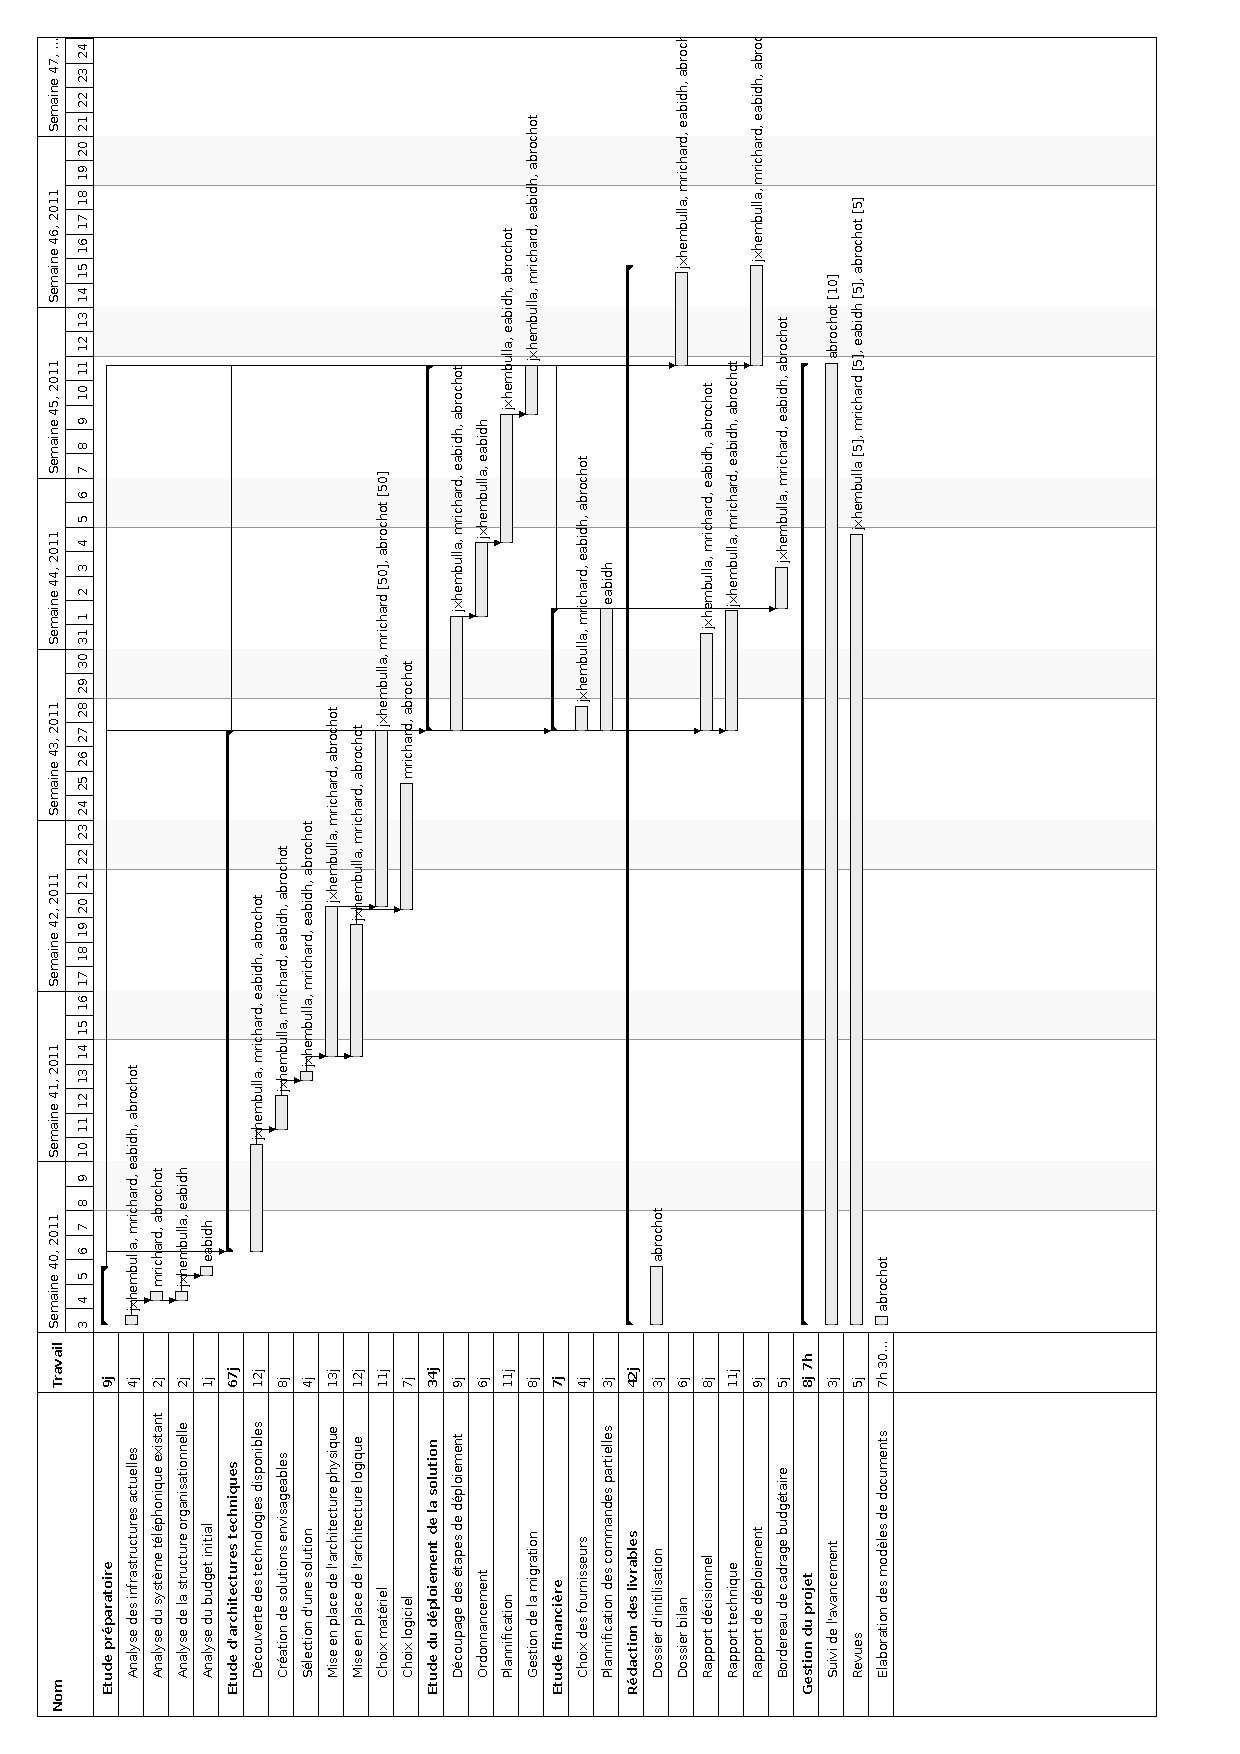
\includepdf{GANTT.pdf}
\newpage
\section{Organisation de l'équipe projet}

\section{Présentation des rôles}
\section{Diagramme de répartition de la charge au sein du groupe}
\end{document}
